%!TeX root = ../main.tex
\section*{Guest Lecture 2a, 13/03/2018}
These lectures will discuss Chern-Simons theory.
This is a $3$-dimensional gauge theory of a Lie-algebra valued $1$-form $A$, with action
\begin{align*}
S &= \frac{k}{4 \pi} \int \tr \left( A \wedge dA + \frac{2}{3} A \wedge A \wedge A\right)\\
&= \frac{k}{4 \pi} \int \varepsilon^{\mu \nu \sigma} \left[A_{\mu a} \partial_\nu A_\sigma^a + \frac{2}{3} f_{abc} A_\mu^a A_\nu^b A_\sigma^c \right] d^3x.
\end{align*}
The explicit appearance of $\varepsilon$ means that this theory is not invariant under \me{one of (?)} $P$ or $T$.
Today we just focus on the Abelian case, where the second term vanishes.

We can consider an action of the form
\[
S_{\text{TOT}} = S_{\text{YM}} + S_{\text{CS}} = \frac{1}{4g^2} \int \tr F \wedge F + S_{\text{CS}}.
\]
Recall some (semiclassical because there might be quantum anomalies) dimensional analysis.
In 4D $g^2$ is dimensionless (except really not because it depends on the energy scale via dimensional regularization) while in 3D it has dimensions of mass.
There are two ways to remember this: one is that
\[
D_{\mu} = \partial_\mu + i A_\mu
\]
so that $A_\mu$ has dimensions of mass, and look at the action $(4g^2)^{-1} \int F^2 \,d^3x$.
\me{There was also a mention of the Ahoromov-Bohm phase $e^{i q \oint A_\mu d^\mu x}$.}

In the low energy limit, $g^2 \to \infty$, so we can forget about the YM terms in the action, so the CS term dominates the IR physics.
Furtheromre, the first term in the CS action is more important.

\subsection*{Quantum Hall Effect}
There is both an integer effect (understood) and a fractional one (an open problem.)
We see how Chern-Simons applies to them.

Classically, the setup is as follows.
We have a 2D thin-film sample in a STRONG (order of teslas) magnetic field, with a voltage $V_y$ in the $y$ direction and a current $I_x$ in the $x$ direction.
The resistivity is $\rho_H = V_y/I_x$.
If the charge carriers have charge $q$, density $n$, and velocity $v_x$, then
\[
\frac{V_y}{I_x} = \frac{E_y L}{J_x L} = \frac{E_y}{J_x}
\]
Since the current density is $J_x = nq v_x$,
\[
\rho_H = \frac{E_y}{n q v_x} = \frac{B}{nq}
\]
as things balance out with the magnetic force.
More generally there is a resistivity \emph{matrix} $\rho_{ij}$ with $\rho_{ij} J_j = E_i$, and we can ask what the values of $\rho_{ij}$ are.

This is a plot of $\rho_{xy}$ in units of $h/e^2$:
\begin{center}
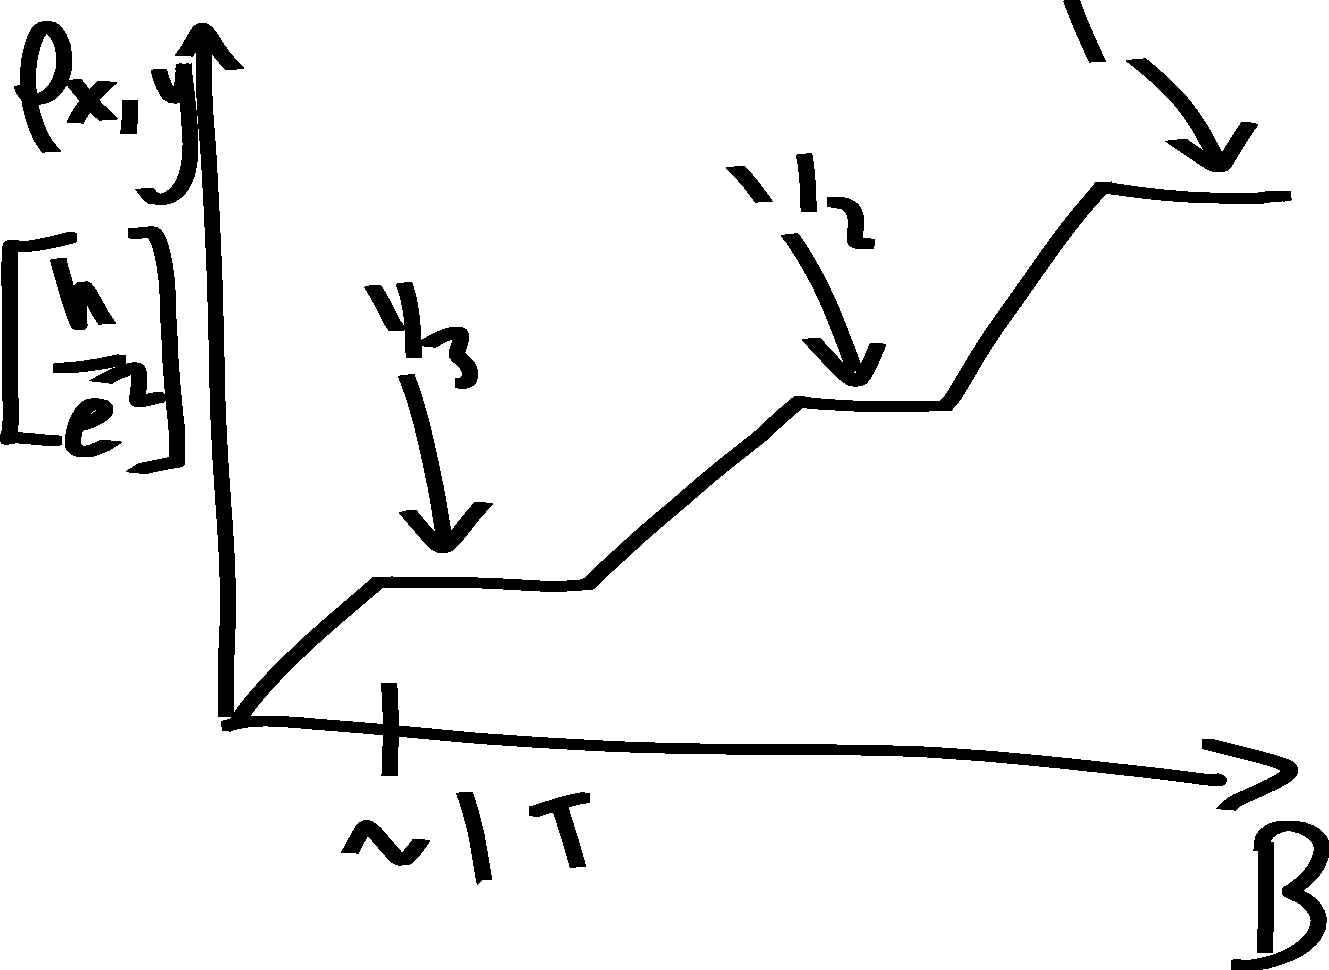
\includegraphics[width = 5in]{fig/quantum-hall-graph.pdf}
\end{center}
$\rho_{xx}$ on the other hand is roughly the same valueof $\rho_{xy}$, but it falls to zero at the plateaus.
This reflects an ``incompressible quantum state.''

This can be explained as follows: \me{(but note that I missed some parts of the following)} Suppose there's a single particle of charge $q$.
We get gapped states each with large degeneracy, via $\hbar \omega_B = q B/m$.
In particular, each particle takes fundamental flux $\phi_0 = 2 \pi \hbar / |e|$, so the total number of states at each energy is
\[
\frac{BA}{\phi_0}
\]
where $A$ is the area of the sample.
Idea is that each state has a ``bubble'' of flux around it and these don't overlap.
The plateaus happend because disorder/impurities spread out the degneracies.
The edges of these spreads are localized nonconductive states, so the first and last part of the increase in $B$ doesn't create any more conductivity.

The \emph{fractional} effect is more mysterious and more difficult to get.
It happens for fractions of the form $n/(2mn \pm 1)$.
It's mostly open why it happens.
One reason is that it depends heavily on the electron-electron interactions.
There are lots of these: if $\nu = 1/3$ then there are something like $\binom{N}{N/3}$ states, which is a \emph{lot.}

\subsection*{Connection to field theory}
Let $A = A_{\text{ext}}$ be the background EM field, with $\mathbf B = B \hat z$ and $\mathbf E = V_y \hat y$.
We write $\psi$ for the electrons in the sample.
Consider a partition function of the form
\[
\int e^{-\frac{i}{\hbar} S[A, \psi)]}.
\]
Here the effective action is
\[
S = \frac{k}{4 \pi} \int A \wedge dA
\]
This is topological, so how does it come from a condensed matter system?
It's reasonable if there are no propagating degrees of freedom.

We have
\[
\left \langle J_i(X) \right \rangle_A = \left \langle \frac{\delta S}{\delta A(x)} \right \rangle = \int \left( \frac{\delta S}{\delta A} e^{\frac{i}{\hbar} S}\right) \mathcal D \psi = \frac{\hbar}{i} \frac{\delta}{\delta A} \int e^{\frac{i}{\hbar} S} \mathcal D \psi = \frac{\delta}{\delta A} \left( e^{\frac{iS}{\hbar}} \right)
\]
so that
\[
\left \langle J_i \right \rangle =\frac{\delta S}{\delta A} = \frac{k}{2 \pi} \varepsilon_{ijk} F_{jk}
\]
Macroscopically, $J_i = k \varepsilon_{ij} E_j /2 \pi$, so $\sigma_{xy} = k/2 \pi$ and $\rho_{xy} = 2 \pi /k$ (where $\hbar = e = 1$.)

We now put the theory on a $2$-torus, so that
\[
S = \frac{k}{4 \pi} \int A \wedge dA = \frac{k}{4 \pi} \int (A_2 A_1 - A_1 A_2) \intd t \intd x \intd y = \frac{k}{2 \pi} \int A_2 \dot A_1 + \text{boundary terms} \intd t \intd x \intd y
\]\
and impose the gauge $A_0 = 0$.

There is one problem here: we still have a equation from varying $A_0$ that we'd now leave out, so we include it manually:
\[
0 = \frac{\delta S}{\delta A_0} = F_{12}.
\]
This means there's no field strength!

Furthermore, there are topological obstructions that can't be gauged away, namely the winding numbers
\[
\frac{1}{2 \pi} \oint_{C_i} A_i \intd x^i
\]
where $C_1, C_2$ are noncontractable loops around the torus.